\section{HTML模板和导入D3}

\begin{minted}[frame=lines,framesep=2mm,baselinestretch=1.2,fontsize=\footnotesize,linenos]{html}
<!DOCTYPE html>
<html lang="en">
  <head>
    <meta charset="UTF-8" />
    <meta name="viewport" content="width=device-width, initial-scale=1.0" />
    <title>D3.js</title>
  </head>
  <body>
    <p>Hello, World! --1</p>
    <p>Hello, World! --2</p>
  </body>
</html>
\end{minted}

这便是最基础的一个HTML文件,可将其命名并保存为\verb|index.html|,在浏览器中打开,可知会打印出两行``Hello, World!''。但现在还没有引入D3,我们要怎么样引入D3,并让D3对该HTML发挥作用呢?

这里,我将之前下载安装好的\verb|d3.js|或\verb|d3.min.js|存放在新建的\verb|js|文件夹下,而\verb|index.html|与该文件夹同级。即文件目录情况为:

\begin{minted}[frame=lines,framesep=2mm,baselinestretch=1.2,fontsize=\footnotesize,linenos]{html}
|-  index.html
|-  js/
        d3.js
        d3.min.js
\end{minted}

将文件安置在相对目录后可从VS Code中打开项目进行编辑。如下为引入了D3的HTML文件\verb|index.js|,只需通过添加一行\verb|<script src="xxx">|来引入即可,\verb|src=|可指定D3.js的存放位置。如我在这里使用的是\verb|d3.min.js|,通过相对目录\verb|./js/d3.min.js|引入。

\begin{minted}[frame=lines,framesep=2mm,baselinestretch=1.2,fontsize=\footnotesize,linenos]{html}
<!DOCTYPE html>
<html lang="en">
  <head>
    <meta charset="UTF-8" />
    <meta name="viewport" content="width=device-width, initial-scale=1.0" />
    <title>D3.js</title>
    
    <!-- 引入D3 -->
    <script src="./js/d3.min.js" charset="utf-8"></script>

  </head>
  <body>
    <p>Hello World! --1</p>
    <p>Hello World! --2</p>
  </body>
</html>

<script>
    var e = d3.select("body").selectAll("p");
    e.style("color","blue").style("font-size","72px");
</script>
\end{minted}

如我使用VS Code打开该项目,并安装了``Preview on Web Server''插件,便可实时地在侧边栏中看到该HTML的展示效果,非常方便。如\figref{fig:open_in_vscode}中所示。通常,在编写Web应用时会利用 \verb|console.log()| 等方法进行调试,则可选择在浏览器中打开,进入到浏览器的开发者调试模式(通常通过F12进入),查看 console 输出、HTML元素信息等。

\begin{figure}[htbp]
    \centering
    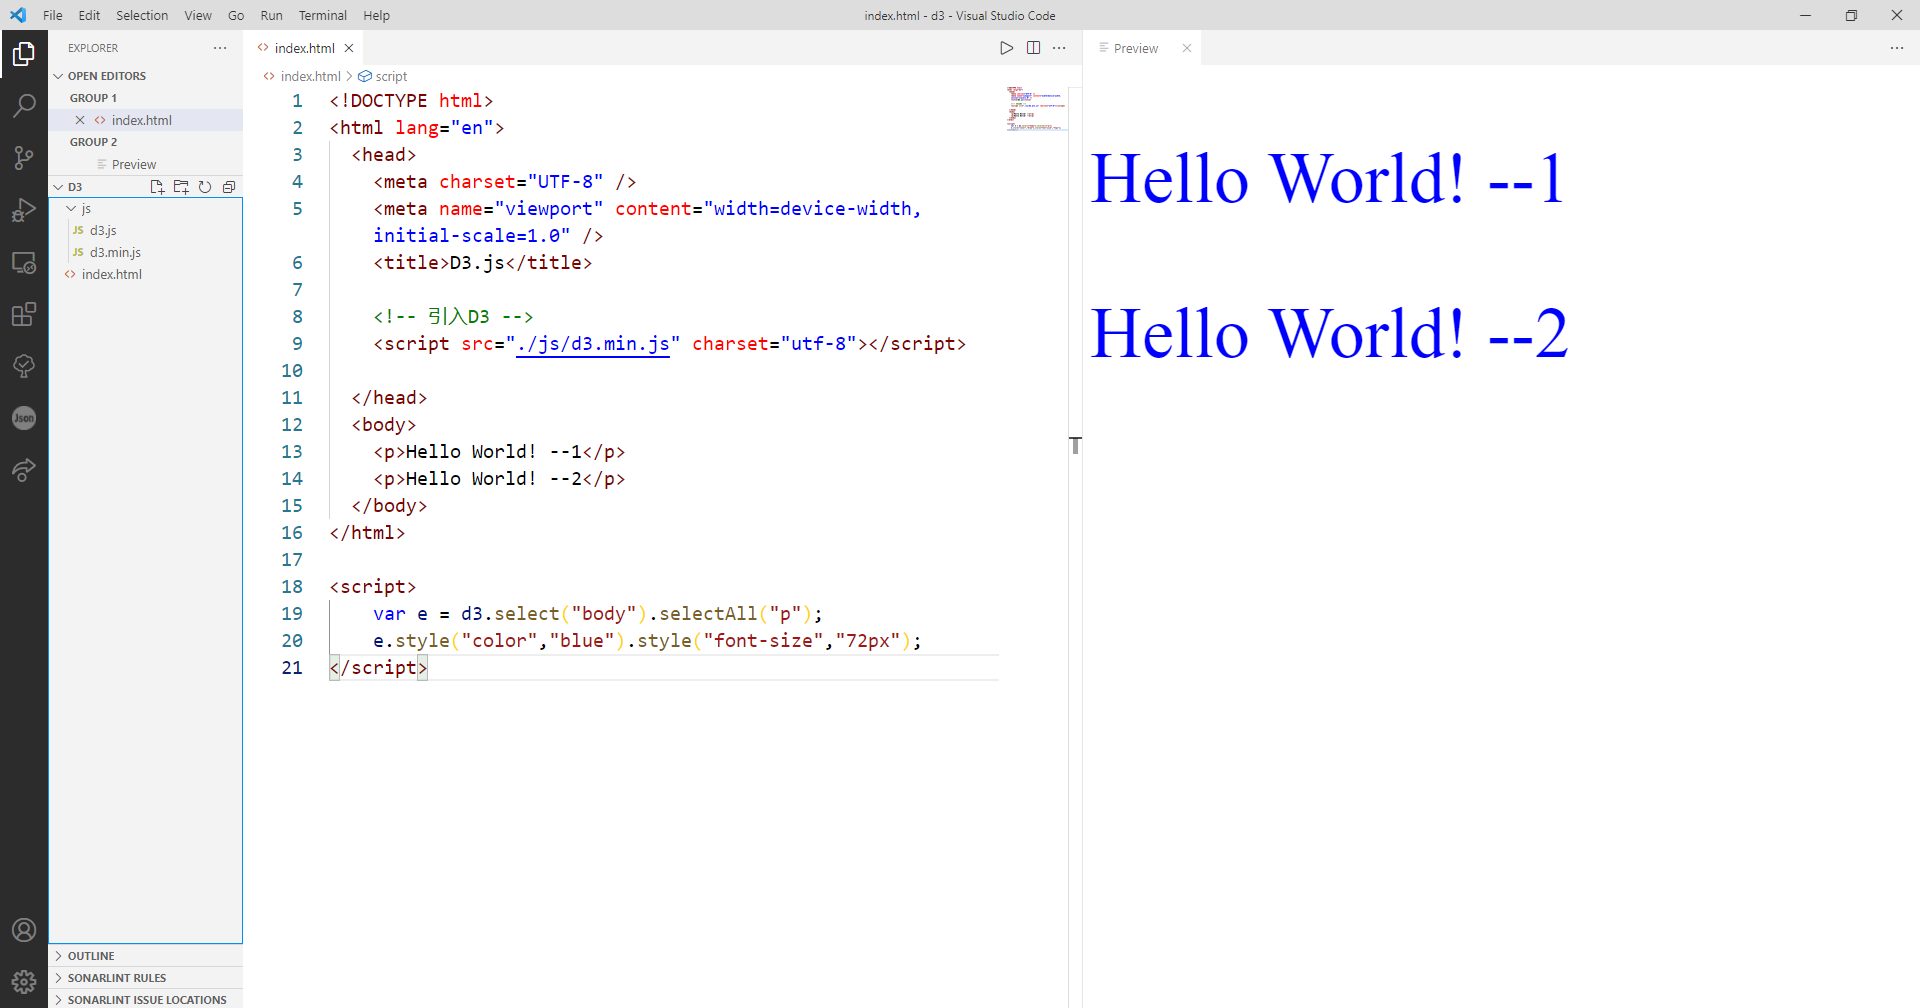
\includegraphics[width=0.9\textwidth]{figure/D3/open_in_vscode.png}
    \caption{\textbf{在VS Code中打开引入了D3操作的项目}}
    \label{fig:open_in_vscode}
\end{figure}

以上导入了D3对p标签文本进行操作后的效果,两行``Hello,World!''变为了蓝色,且字号变大了许多。这是通过用D3的script脚本来控制的,而这些script我在以上代码片段中写在了该html文件的末尾被\verb|<script>...</script>|标签(HTML中标签总是成对出现)包围起来的部分,也可以单独保存为一个js文件,通过类似于D3导入的方式引用。

\section{元素选择和数据绑定}

我们再观察上述\verb|<script>|中的D3代码:

\begin{minted}[frame=lines,framesep=2mm,baselinestretch=1.2,fontsize=\footnotesize,linenos]{javascript}
var e = d3.select("body").selectAll("p");
// 选择所有 <p> 标签的网页元素
e.style("color","blue").style("font-size","72px");
// 将颜色样式改为 blue,用链式语法继续将文本大小修改为 72px
\end{minted}

\subsection{元素选择}

D3可以非常简洁地操作HTML中的DOM元素,我们通过\verb|d3.select()| (选择第一个找到的元素)或 \verb|d3.selectAll()|(选择所有找到的元素) 选择元素后返回了对象,这就是选择集。我们可以根据元素的不同特性来选择出想要的对象,根据属性值、class、ID等都可以进行选择。

而多次连续调用的\verb|.style()|等函数被称为链式语法,和JQuery中的语法颇为类似。此处我们调用\verb|.style()|改变了元素的样式,而D3还可以提供设置属性(\verb|.attr()|)、添加(\verb|.append()|)、更改文本内容(\verb|.text()|)等方法,能满足用户大部分的需求。

\subsection{数据绑定}

D3可以将数据绑定到DOM上去(DOM能将HTML文档表达为树结构,数据绑定与DOM绑定即是让HTML标签与数据进行绑定)。比如,让的段落元素p标签与字符串变量``Hello''绑定,绑定后,当需要依靠该数据操作元素时,会更为方便。

D3中有两个函数可以绑定数据:

\begin{enumerate}
    \item \verb|datum()|:绑定一个数据到选择集上。
    \item \verb|data()|:绑定一个数组到选择集上,数组的各项值分别与选择集的各元素绑定。(更常用)
\end{enumerate}

举一个例子,当前有三个段落元素如下:

\begin{minted}[frame=lines,framesep=2mm,baselinestretch=1.2,fontsize=\footnotesize,linenos]{html}
<body>
    <p>张三</p>
    <p>李四</p>
    <p>王五</p>
</body>
\end{minted}

方式一:使用\verb|datum()|绑定。假设有一个字符串``China'',可将其分别与三个段落p元素绑定:

\begin{minted}[frame=lines,framesep=2mm,baselinestretch=1.2,fontsize=\footnotesize,linenos]{javascript}
var str = "China";
var body = d3.select("body");
var p = body.selectAll("p");
p.datum(str);
p.text(function(d, i){
    return i +": "+ d;
});
\end{minted}

绑定数据后,使用此数据来修改三个段落元素的内容,其结果为:

\begin{minted}[frame=lines,framesep=2mm,baselinestretch=1.2,fontsize=\footnotesize,linenos]{html}
0: China
1: China
2: China
\end{minted}

在上面的代码中,用到了一个匿名函数\verb|function(d, i)|。当选择集需要使用被绑定的数据时,常需要这么使用。其包含两个参数,其中d代表数据,即与某元素绑定的数据,而i 代表索引,代表数据的索引号,从 0 开始。

方式一:使用\verb|data()|绑定。有一个数组\verb|var arr = ["a", "b", "c"];|,接下来要分别将数组的各元素绑定到三个段落元素上。

绑定后,其对应关系应为张三-a,李四-b,王五-c。我们调用\verb|data()|函数 绑定数据,并替换三个段落元素的字符串为被绑定的字符串,代码如下:

\begin{minted}[frame=lines,framesep=2mm,baselinestretch=1.2,fontsize=\footnotesize,linenos]{javascript}
var arr = ["a", "b", "c"];
var body = d3.select("body");
var p = body.selectAll("p");
p.data(arr).text(function (d, i) {
  return d;
});
\end{minted}

此处也用到了一个无名函数 \verb|function(d, i)|,其对应的情况为i=0, 1, 2时,d分别为a, b, c。

此时,三个段落p元素与数组 arr 的三个字符串是一一对应的。因此,在函数  \verb|function(d, i)| 直接 \verb|return d| 即可。

\section{插入和删除元素}

\subsection{插入元素}

插入元素涉及的函数有两个,分别是:

\begin{enumerate}
    \item \verb|append()|:在选择集末尾插入元素
    \item \verb|insert()|:在选择集前面插入元素
\end{enumerate}

假设有和前文一样的三个段落p元素:张三、李四、王五,其中给李四用id加了标签\verb|id="label"|。

\begin{minted}[frame=lines,framesep=2mm,baselinestretch=1.2,fontsize=\footnotesize,linenos]{html}
<body>
    <p>张三</p>
    <p id="label">李四</p>
    <p>王五</p>
</body>
\end{minted}

\begin{minted}[frame=lines,framesep=2mm,baselinestretch=1.2,fontsize=\footnotesize,linenos]{javascript}
var body = d3.select("body");
body.append("p").text("赵六")
// 在 body 的末尾 append p 元素
body.insert("p","#label").text("insert here")
// 找到 id 为 label 的标签 p,insert 插入元素
\end{minted}

最终结果为:

\begin{minted}[frame=lines,framesep=2mm,baselinestretch=1.2,fontsize=\footnotesize,linenos]{javascript}
张三
insert here
李四
王五
赵六
\end{minted}

与预想的一致,即\verb|append()|在末尾插入,\verb|insert()|在元素前插入。

\subsection{删除元素}

删除一个元素时,对于选择的元素,使用 \verb|remove()| 函数即可,例如:

\begin{minted}[frame=lines,framesep=2mm,baselinestretch=1.2,fontsize=\footnotesize,linenos]{javascript}
var p = body.select("#label");
p.remove();
\end{minted}

于是,便删除了指定 id 的段落元素。

\section{enter()和exit()方法}

使用 D3 中的\verb|enter()|和\verb|exit()|对象选择方法,可以为传入的数据(通常为数组形式)创建新节点,以及删除不再需要的传出节点。

当数据绑定到选择集上后,数据数组中的每个元素都与选择中的相应节点配对。 如果节点数少于数据的长度(即该数组的长度),则额外的数据元素可通过\verb|enter()|选择,附加进节点。 如果节点数多于数据的长度,通过\verb|exit()|选择,多余的节点会被删除。下面通过代码来说明。

假设当前有2个段落标签,其中的内容分别是a和b。

\begin{minted}[frame=lines,framesep=2mm,baselinestretch=1.2,fontsize=\footnotesize,linenos]{html}
<body>
    <p>a</p>
    <p>b</p>
</body>
\end{minted}

我们考察以下三种情况:不使用\verb|enter()|和\verb|exit()|,使用\verb|enter()|,和使用\verb|exit()|来观察其它们两个的作用。

\begin{minted}[frame=lines,framesep=2mm,baselinestretch=1.2,fontsize=\footnotesize,linenos]{javascript}
// Case 1: Update
var p =  d3.select("body")
  .selectAll("p")
  .data([1, 2, 3, 4])
    .text(function(d) { return d; });
// 结果为 1 2
// 即a和b被替换成了数组的中的前两个元素

// Case 2: Enter
p.enter().append("p")
    .text(function(d) { return d; });
// 结果为 1 2 3 4
// 在 Case 1 的基础上继续操作
// 数据长度大于节点数,通过enter(),3和4成为了附加节点

// Case 3: Exit
d3.select("body")
  .selectAll("p")
  .data([8])
  .exit().remove()
    .text(function(d) { return d; });
// 结果为 1
// 在 Case 2 的基础上继续操作
// 数据长度小于节点数,通过exit(),删除了多余节点,留下了1
// 注:如果先.text,再.exit().remove(),则会因为先赋值了而结果为8
\end{minted}

通过分别处理这三种情况,我们可以观察和分析了解了这二者的作用。可以认识到各个操作具体作用于了哪些节点。这在绘制图形时可以得到应用——如对于条形图,我们可能先使用了旧的尺度来初始化了输入的条的个数,当遇到新的输入导致数据长度与初始化时的条数不一致时,就可以通过这二者来进行更新。